\exo \textbf{Synthèse du paracétamol}

\vspace{0.3cm}

Le paracétamol est un médicament qui se rapproche de l'aspirine par ses propriétés analgésiques et antipyrétiques. On l'obtient par réaction entre le paraaminophénol et l'anhydride éthanoïque. L'autre produit
de la réaction est l'acide éthanoïque.

\begin{figure}[h]
\begin{center}
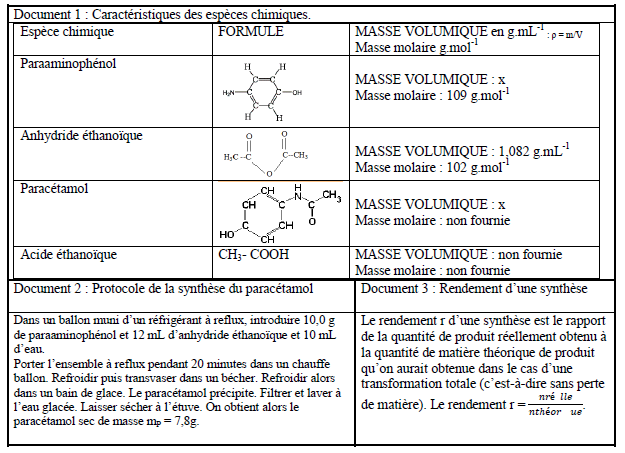
\includegraphics[width=\columnwidth]{images/Exo4_Document_123}
\end{center}
%\caption{\label{fig:Spectre_Absorption_Mercure}Spectre simplifié d'absorption du Mercure}
\end{figure}

\vspace{0.3cm}

\textbf{Document $4$ :} masse molaire des atomes.

$$M(H) = 1,0\text{ }\gram.\mole^{-1}\text{; }M(C)=12,0\text{ }\gram.\mole^{-1}\text{; }M(N)=14,0\text{ }\gram.\mole^{-1}\text{; }M(O)=16,0\text{ }\gram.\mole^{-1}$$

\vspace{0.3cm}

\textbf{Généralités sur le protocole de synthèse}

\begin{enumerate}
\item Légender le schéma expérimental ci-dessous.
\item Pour quelle raison doit-on refroidir le mélange obtenu à la fin de la synthèse ?
\end{enumerate}

\begin{figure}[h]
\begin{center}
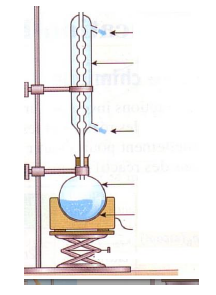
\includegraphics[width=0.25\columnwidth]{images/Exo4_Schema_Experimental}
\caption{\label{fig:Schema_Exp}Schéma expérimental à compléter}
\end{center}
\end{figure}

%\vspace{0.3cm}

\newpage

\textbf{Bilan quantitatif de la synthèse}

\begin{enumerate}
\item L'équation de la réaction de synthèse est:

\begin{chemmath}
C_{6}H_{7}ON + 2C_{4}H_{6}O_{3} + H_{2}O \longrightarrow C_{8}H_{9}O_{2}N + 3C_{2}H_{4}O_{2}
\end{chemmath}

Relier les formules brutes de cette équation aux noms des réactifs est des produits de cette synthèse.

\item Calculer les quantités de matières initiales des réactifs (l'eau est supposée en excès : on ne calculera
donc pas sa quantité de matière ; elle sera notée en excès dans le tableau d'avancement).

\item Etablir le tableau d'avancement de la réaction.

\item Déterminer l'avancement maximal xmax. Le mélange initial est-il dans les proportions
stœchiométriques ? Justifier.

\item En déduire la quantité de matière $n_{P}$ (théorique) de paracétamol qu'on obtiendrait si la réaction était totale.

\item Calculer la quantité de matière $n_{P}$ (réelle) de paracétamol réellement obtenu à l'issue du protocole.

\item Quel est le rendement de la synthèse du paracétamol ?

\end{enumerate}

\vspace{0.3cm}